For the purpose of this thesis, geometry will be restricted to how points, lines, planes (and higher dimensional objects) interact with space. To build a bridge between algebra and geometry, there must be an established way to discuss geometry algebraically. This is where the concepts of affine spaces comes in.  

\subsubsection{Affine Spaces}
\label{sssec:affine-spaces}
Let us take a moment to reflect around how one might represent a geometric object. Consider a line. One could use the well known two dimensional cartesian plane, plot the points $(x_1,y_1), (x_2,y_2)$ and then pull a pen between the two points. Here, a line as been created, but it is dependent on the following: a coordinate system and a restriction of dimension so we can physically represent it. These restrictions are undesirable when studying a line algebraically, so we must circumvent these restrictions. The solution is affine spaces. Affine spaces are coordinate-agnostic spaces. This eliminates our need for the coordinate system that was a prerequisite when drawing the lines, which is a good start. The affine space is also easily extended beyond the physical. 

\begin{definition}
    An \textit{affine space} is either the empty set, or a triple $\ideal{ E, \vec{E}, +}$. $E$ is a nonempty set of points while $\vec{E}$ is a vector space (of translations). The action $+$ is an operation on both $E$ and $\vec{E}$ defined as follows: $+: E \times \vec{E} \rightarrow E$. The following axioms are assumed for affine space:
    \begin{enumerate}
        \item $a + 0 = a$ for every $a \in E$.
        \item $(a + u) + v = a + (u + v)$ for every $a \in E$ and every $u,v \in \vec{E}$.
        \item For any two points $a,b \in E$, there is a unique $u \in \vec{E}$ such that $a + u = b$
    \end{enumerate}
\end{definition}

\begin{figure}[ht]
    \centering
    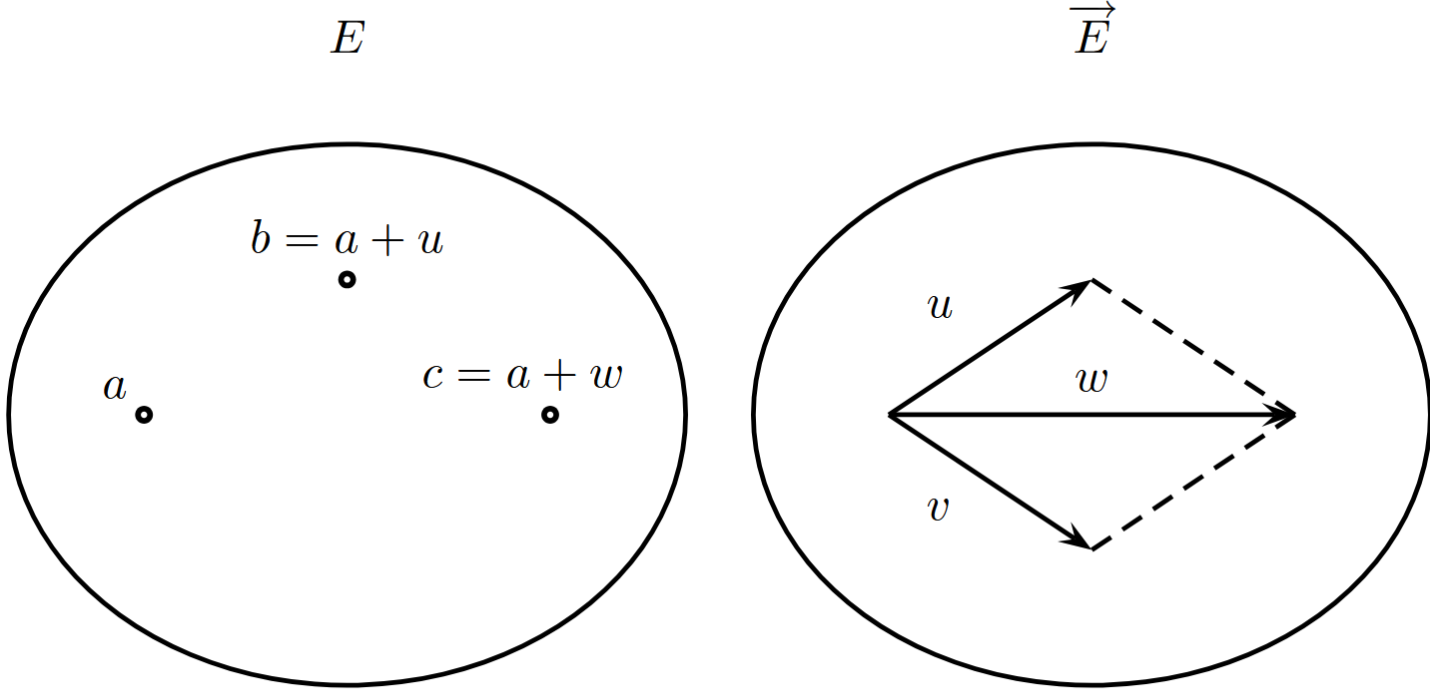
\includegraphics[width = \textwidth]{figures/AffineSpace.png}
    \caption{Intuitive understanding of affine space \cite{gallier2025affine}}
    \label{fig:affine-space}
\end{figure}

A quick note of importance on each axiom. If you start at point a and do nothing, you should still be at a.  Axiom two deals with the associative property. The ability to rearrange calculations simplifies any algebra involved. The last axiom, that of uniqueness is computationally useful. Assuming that an unique element in $\vec{E}$ always exists that can connect two points $a$ and $b$ is useful when solving these problems on a higher level of abstraction, especially when a computer that cannot handle errors is involved. 

The intuition behind the coordinate-agnostic nature should be clear when considering figure \ref{fig:affine-space}. Here a seperation between the vectors and the points \textit{to which the vector is applied to} should be noted. These two can be defined independently and therefore there is no system tying them together.An example is provided for further clarity.

\begin{example}\label{def:affine-space}
    Given a field $k$ and a positive integer $n$, define the $n$-dimensional \textit{affine space} over $k$ as:
    \[
         k^n := \ideal{\left\{[\vectorComponents{\hat{x}}]^T : \hat{x_i} \in k, i=1,\dots, n\right\}, \vec{k^n}, +}
    \]
    Where $\vec{k^n}$ is the vector space of translations, and $+$ denotes the action of shifting a point by a vector via component-wise addition.
\end{example}

To further our understanding of the space, we can use the concrete example where the field in question is $\R$. Then, we get the familiar space $\R^n$ . So the affine space is more abstract than the one we are used to dealing with from real world applications where we are restricted. 

\subsubsection{Polynomials in Affine Spaces}    
\label{sssec:polynomials-in-affine-spaces}

With a better undestanding of affine spaces, we will consider how polynomials relate to this space. Using the definition \ref{def:polynomial} we define the polynomial \textit{function} $p \in \polyRing$ as follows: 

\[
    p : k^n  \rightarrow k
\]

The function maps the multidimensional field onto the single dimension. This $p$ takes every $\vectorComponents{x}$ and replaces it with $\vectorComponents{a} \in \polyRing$. This is done easily by substituting every $x_i = a_i$ in the polynomial $p$. Since all the subbed in $a$'s are elements $\polyRing$, then $p(\vectorComponents{a})$ is also in $\polyRing$.

\subsubsection{Affine Varieties}
\label{sssec:affine-varieties}
With an understanding of how the space we will operate upon will work and how the polynomials can be evaluated on that space, the first algebraic structure of geometry will be discussed: affine varieties.  

\begin{definition}
    Let $k$ be a field, and let $\vectorComponentsX{f}{s}$ be polynomials in $\polyRing$. Then, set
    \[
        \boldsymbol{V}(\vectorComponentsX{f}{s}) = 
        \left\{
            (\vectorComponents{a}) \in k^n |\enspace f_i(\vectorComponents{a}) = 0 \enspace \forall 1 \leq i \leq s
        \right\}
    \]
    We call $\boldsymbol{V}(\vectorComponentsX{f}{s})$ the \textbf{affine variety} defined by $\vectorComponentsX{f}{s}$.
\end{definition}

\begin{figure}[ht]
    \centering
    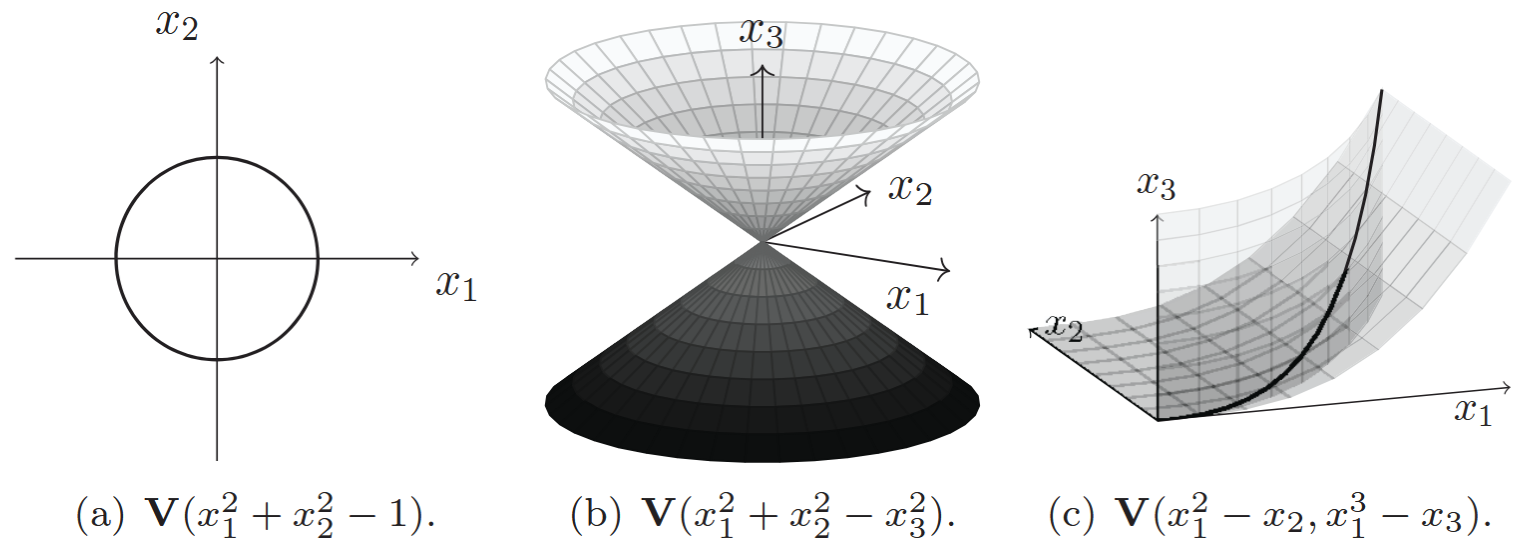
\includegraphics[width = \textwidth]{figures/AffineVariety.png}
    \caption{Examples of affine spaces \cite{Applied}}
    \label{fig:variety-example}
\end{figure}

In other words, the affine variety is the set of $(\vectorComponents{a})$ that solve all the equations defined in the variety simultaneously. Or, it is the intersection of all the polynomial roots. Even though $\boldsymbol{V}$ might simply look like a graphed equation, figure \ref{fig:variety-example}a only provides the \textit{base} for intuition. While it may look like a regular circular graph, with familiar $x$ and $y$ coordinates, the keen observer will note that we are dealing with two dimensions, $x_1, x_2$ and that the graph is in fact the where this polynomial studied is equal to $0$. If we extract the polynomial from the variety and set it to $0$, we end up with $x_1^2 + x_2^2 = 1$. Figures \ref{fig:variety-example}b and \ref{fig:variety-example}c show the increasing complexity in three dimensions. Graphing this equation makes the roots of the polynomial self-evident, but graphing it is neither necessary or desirable. It is only a tool to inform intuition. This is especially true as we are interested in $n$ dimensions and graphing will become next to impossible.